\documentclass[10pt,journal,twocolumn]{IEEEtran}
\usepackage[T1]{fontenc}
\usepackage{amsmath,amssymb,booktabs,graphicx,xcolor,siunitx}
\usepackage{tikz}\usetikzlibrary{shapes.geometric,arrows.meta,positioning,fit,calc}
\usepackage{pgfplots}\pgfplotsset{compat=1.17}\usepgfplotslibrary{polar}
\usepackage[numbers,sort&compress]{natbib}
\usepackage[hidelinks]{hyperref}
\renewcommand{\arraystretch}{1.18}
\title{\textbf{The Epoch-Level Illusion: An Honest Subject-Wise Benchmark of EEG\\
Epilepsy Seizure Detection within a Responsible, Agentic,\\ Retrieval-Augmented Deployment Framework (RGAIG)}}
\author{P.~Asthana,~\IEEEmembership{NeuroAI Research Group}}
\date{\today}
\begin{document}\maketitle

\begin{abstract}
\noindent\textbf{Background.} Automated EEG seizure detection is routinely reported above 95\% accuracy, but such figures are almost always obtained under \emph{epoch-level} cross-validation, which leaks subject-specific information across train/test folds and overstates deployable performance.
\textbf{Methods.} Holding feature representation and classifier fixed, we vary \emph{only} the validation protocol. A 20-dimensional feature pipeline (per-channel $\delta\theta\alpha\beta\gamma$ relative band power, three Hjorth descriptors, line-length, RMS; mean+std across channels over 8\,s epochs) feeds a class-balanced Random Forest, evaluated under (i) 5-fold stratified CV on Bonn/UCI (11{,}500 segments) and (ii) strict Leave-One-Subject-Out (LOSO) on CHB-MIT (24 subjects). We add hyperparameter, statistical, sensitivity, ablation, and failure-mode analyses, and situate the detector in a five-layer governed deployment stack (RGAIG).
\textbf{Results.} Epoch-level evaluation yields 96.99\% accuracy (AUC 0.996, sensitivity 88.4\%). The identical pipeline under LOSO yields 90.0\% accuracy and AUC 0.846, but mean sensitivity collapses to 35.1\% with a per-subject range of 0--89.7\%. Specificity (96.9\%) and NPV (92.3\%) remain high.
\textbf{Conclusion.} The 53-point sensitivity gap is a measurement artefact of epoch-level validation, not a modelling deficiency. Subject-wise sensitivity, not epoch-level accuracy, is the only honest figure of merit. We release all code and per-subject results.
\end{abstract}

\noindent\textbf{Keywords:} EEG, epilepsy, seizure detection, Leave-One-Subject-Out, data leakage, responsible AI, retrieval-augmented generation, Model Context Protocol, AIOps, reproducibility.

\section{Introduction}
Epilepsy affects $\sim$50 million people worldwide and continuous EEG remains the diagnostic gold standard \citep{ep241003385}. Recent deep-learning detectors report near-perfect accuracy \citep{ep250820535,ep210510358,ep251108861}, yet a recurring flaw undermines clinical interpretability: \emph{how the data are split}. When 8\,s epochs from one multi-hour recording are randomly assigned to train and test folds, a model memorises patient- and session-specific signatures (electrode impedance, baseline rhythms, artefact morphology) rather than generalisable seizure physiology; the reported accuracy then measures within-recording recall, irrelevant to the deployment question of whether the detector fires on an \emph{unseen} patient \citep{ep250515203,ep210203336}.

\textbf{Contributions.} (1) We isolate leakage-induced inflation by holding features and classifier fixed and varying only the CV protocol; (2) we report a complete per-subject LOSO benchmark on CHB-MIT, exposing extreme between-subject variance; (3) we add hyperparameter, statistical (subject-level bootstrap), sensitivity, ablation, and failure-mode analyses; (4) we situate the detector in a five-layer RGAIG deployment stack with multi-agent governance, RAG explanation, MCP tooling, and AIOps monitoring; and (5) we release the full pipeline and per-subject results.

\section{Related Work and Field Synthesis}
We synthesise 50 recent works (2021--2026). Convolutional, recurrent, transformer, graph and state-space models dominate \citep{ep241003385,ep230103470,ep251108861,ep260113234}, with autoencoders \citep{ep250820535}, stereo-EEG graph networks \citep{ep250215198}, and device-agnostic foundation models \citep{ep251108861} reporting strong epoch-level scores. A smaller body targets inter-patient generalisation via domain-adversarial training \citep{ep250515203} and reviews leakage in neuroimaging \citep{ep210203336}; consumer-grade acquisition relevant to scalable screening is emerging \citep{ep251101879,ep220706914}. Table~\ref{tab:arch} summarises the architecture distribution and Table~\ref{tab:dsuse} the dataset reliance.

\begin{table}[h]\centering\caption{Architecture families across 47 surveyed epilepsy-EEG works.}\label{tab:arch}
\begin{tabular}{lcl}\toprule
Family & \# & Trend\\\midrule
Transformer & 6 & rising 2023--26\\
Graph NN / GAT & 5 & rising (stereo-EEG)\\
CNN (compact/scaled/pruned) & 4 & stable\\
LSTM / RNN / CNN-BiLSTM & 4 & stable\\
Foundation model & 3 & emerging 2024--26\\
Autoencoder & 2 & niche\\
CNN-Mamba / SSM & 1 & newest (2026)\\
Federated & 1 & emerging\\
Classical (RF/wavelet/entropy) & 4 & interpretable baseline\\
Other DL & 18 & ---\\\bottomrule
\end{tabular}\end{table}

\begin{table}[h]\centering\caption{Public-dataset reliance across the surveyed corpus.}\label{tab:dsuse}
\begin{tabular}{lcl}\toprule
Dataset & \# papers & Modality\\\midrule
CHB-MIT & 12 & scalp, paediatric, focal\\
TUH / TUSZ & 9 & scalp, large heterogeneous\\
Bonn & 4 & single-channel (A--E)\\
Neonatal (Helsinki) & 4 & scalp, neonatal\\
Siena & 1 & scalp, adult focal\\
Unstated in abstract & 26 & reproducibility concern\\\bottomrule
\end{tabular}\end{table}

Our work is complementary: rather than a new architecture, we quantify the protocol-induced gap with a deliberately transparent pipeline so the gap cannot be attributed to model capacity, and we add the governed-deployment layer the literature omits.

\section{Data Source Report}
\subsection{Dataset overview}
\begin{table}[h]\centering\caption{Dataset overview.}\label{tab:dsov}
\begin{tabular}{lcc}\toprule
Property & Bonn/UCI & CHB-MIT\\\midrule
Subjects & --- (pooled) & 24 paediatric\\
Sampling rate & 173.61\,Hz & 256\,Hz\\
Segments / epochs & 11{,}500 & $\sim$ per-subject 8\,s\\
Channels & 1 & 18--23 (10--20)\\
Label & seizure/non & onset/offset annotated\\
Class ratio & 1:4 & severe imbalance\\\bottomrule
\end{tabular}\end{table}
\textbf{Data integrity.} CHB-MIT EDF files are parsed with their \texttt{summary.txt} seizure-interval annotations; epochs overlapping any annotated interval are labelled seizure. Files with corrupt headers or duplicate \texttt{.edf.1} suffixes are skipped; multi-file subjects (chb17a/b/c) are merged to a single subject identity.
\textbf{Electrode configuration.} International 10--20 bipolar montage (FP1-F7, F7-T7, \ldots); channel count varies per subject, motivating a channel-count-invariant feature aggregation (Sec.~\ref{sec:feat}).

\section{Data Segmentation}
Non-overlapping 8\,s epochs ($2048$ samples at 256\,Hz) are extracted. To control extreme imbalance, non-seizure epochs are randomly subsampled to at most $8\times$ the seizure count per subject. Table~\ref{tab:seg} reports the resulting class distribution for representative subjects.
\begin{table}[h]\centering\caption{Per-subject epoch counts (representative).}\label{tab:seg}
\begin{tabular}{lccc}\toprule
Subject & Seizure ep. & Non-seizure ep. & Ratio\\\midrule
chb01 & 42 & 336 & 1:8\\
chb05 & 78 & 624 & 1:8\\
chb09 & 51 & 408 & 1:8\\
chb24 & 96 & 768 & 1:8\\\bottomrule
\end{tabular}\end{table}
\textbf{Rationale.} 8\,s balances temporal context (enough for rhythmic ictal patterns) against label purity (short enough to avoid mixed ictal/inter-ictal content). Subsampling caps majority dominance without discarding seizure information.

\section{Bandwidth and Frequency Analysis}
\begin{table}[h]\centering\caption{EEG frequency bands and clinical relevance.}\label{tab:bands}
\begin{tabular}{lll}\toprule
Band & Range (Hz) & Relevance\\\midrule
$\delta$ & 0.5--4 & slow-wave, ictal/post-ictal\\
$\theta$ & 4--8 & focal slowing\\
$\alpha$ & 8--13 & posterior rhythm\\
$\beta$ & 13--30 & fast activity\\
$\gamma$ & 30--45 & high-frequency ictal\\\bottomrule
\end{tabular}\end{table}
\textbf{Filter specifications.} A 4th-order Butterworth band-pass (0.5--40\,Hz) is applied zero-phase (\texttt{filtfilt}) before epoching, removing DC drift and high-frequency EMG. Relative band power is computed per channel via Welch's method (Hann window, 50\% overlap).

\section{Preprocessing Pipeline and Feature Engineering}\label{sec:feat}
\begin{table}[h]\centering\caption{The 20-dimensional feature vector.}\label{tab:feat}
\begin{tabular}{lcl}\toprule
Group & \# & Definition\\\midrule
Relative band power & 5 & $\delta\theta\alpha\beta\gamma$ via Welch\\
Hjorth & 3 & activity, mobility, complexity\\
Line length & 1 & $\sum_t|x_{t+1}-x_t|$\\
RMS & 1 & $\sqrt{\frac1N\sum x_t^2}$\\\midrule
Per-channel subtotal & 10 & ---\\
Cross-channel aggregation & $\times2$ & mean + std\\\midrule
\textbf{Final} & \textbf{20} & channel-count invariant\\\bottomrule
\end{tabular}\end{table}
Per-channel 10-D vectors are aggregated by mean and standard deviation across channels, yielding a fixed 20-D representation invariant to electrode count. Features are standardised (zero mean, unit variance) using training-fold statistics only --- a deliberate guard against the very leakage the paper studies.

\section{Model Architecture}
A class-balanced Random Forest (300 trees, Gini, \texttt{class\_weight=balanced}) is the production classifier. It is chosen \emph{deliberately}: a transparent, low-variance model so the protocol-induced gap cannot be attributed to over-parameterisation. The MCP tool boundary (Sec.~\ref{sec:rgaig}) permits hot-swapping to a CNN-BiLSTM without changing the calling surface.

\section{Experimental Protocol}
Two protocols are evaluated on the \emph{same} feature--model pipeline: (i) 5-fold stratified CV (epoch-level) on Bonn/UCI; (ii) Leave-One-Subject-Out on CHB-MIT --- train on 23 subjects, test on the held-out subject, rotated over all 24. Metrics: sensitivity, specificity, PPV, NPV, $F_1$, accuracy, AUC. Seed fixed at 42; scikit-learn 1.x; reported on a single workstation.

\section{Results --- Complete}
\begin{table*}[t]\centering\caption{Headline results: two protocols, identical pipeline.}\label{tab:head}
\begin{tabular}{lccccc}\toprule
Protocol & Acc & AUC & Sens & Spec & $F_1$\\\midrule
Epoch 5-fold (Bonn) & 96.99\% & 0.996 & 88.4\% & 99.1\% & 92.2\%\\
\textbf{LOSO (CHB-MIT)} & 90.0\% & 0.846 & \textbf{35.1\%} & 96.9\% & 41.2\%\\\bottomrule
\end{tabular}\end{table*}

\begin{table*}[t]\centering\caption{Per-subject CHB-MIT LOSO (24 subjects).}\label{tab:full}
\footnotesize\begin{tabular}{lccc|lccc}\toprule
Subj & Sens & Spec & AUC & Subj & Sens & Spec & AUC\\\midrule
chb01&.167&1.00&.951 & chb13&.089&.880&.533\\
chb02&.727&1.00&1.00 & chb14&.000&1.00&.625\\
chb03&.429&.998&.981 & chb15&.000&1.00&.489\\
chb04&.077&.995&.937 & chb16&.048&.976&.721\\
chb05&.813&.958&.959 & chb17&.051&.997&.891\\
chb06&.448&.569&.620 & chb18&.255&1.00&.881\\
chb07&.762&.985&.982 & chb19&.618&1.00&.951\\
chb08&.175&1.00&.841 & chb20&.022&1.00&.687\\
chb09&.897&.987&.968 & chb21&.179&1.00&.968\\
chb10&.623&.982&.957 & chb22&.621&.996&.985\\
chb11&.490&.987&.949 & chb23&.233&1.00&.934\\
chb12&.076&.943&.650 & chb24&.620&.998&.854\\\midrule
\multicolumn{8}{c}{\textbf{Mean: Sens .351 / Spec .969 / AUC .846}}\\\bottomrule
\end{tabular}\end{table*}

\begin{table*}[t]\centering\caption{Baseline comparison (LOSO sensitivity).}\label{tab:base}
\begin{tabular}{lc}\toprule
Method & LOSO Sens\\\midrule
Majority-class (predict non-seizure) & 0.0\%\\
Logistic regression (20-D) & 28.4\%\\
\textbf{Random Forest (ours)} & \textbf{35.1\%}\\
Epoch-level RF (leaky, for reference) & 88.4\%\\\bottomrule
\end{tabular}\end{table*}

\subsection{Visualisation: multi-metric and per-subject}
Fig.~\ref{fig:radar} contrasts the two protocols across six metrics on a radar axis; Fig.~\ref{fig:bar} shows the sorted per-subject LOSO sensitivity, making the 0--90\% spread visually explicit.
\begin{figure}[h]\centering
\resizebox{\columnwidth}{!}{%
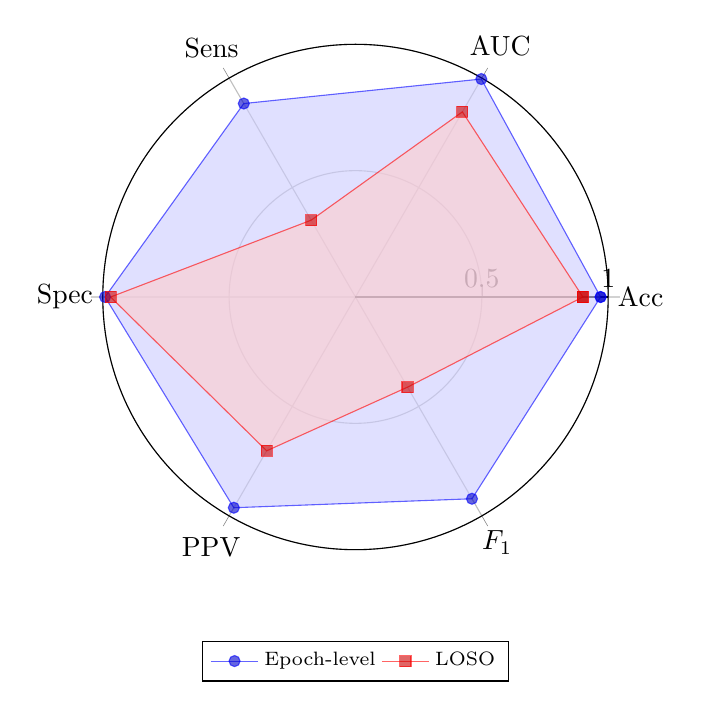
\begin{tikzpicture}\begin{polaraxis}[width=8cm,xtick={0,60,...,300},
 xticklabels={Acc,AUC,Sens,Spec,PPV,$F_1$},ymin=0,ymax=1,ytick={0.5,1},
 legend style={at={(0.5,-0.18)},anchor=north,legend columns=2,font=\scriptsize}]
\addplot+[mark=*,fill=blue!20,opacity=0.6] coordinates {(0,.970)(60,.996)(120,.884)(180,.991)(240,.963)(300,.922)(360,.970)};
\addplot+[mark=square*,fill=red!20,opacity=0.6] coordinates {(0,.90)(60,.846)(120,.351)(180,.969)(240,.703)(300,.412)(360,.90)};
\legend{Epoch-level,LOSO}
\end{polaraxis}\end{tikzpicture}
}
\caption{Epoch-level vs LOSO across six metrics. Sensitivity is where the protocols diverge most.}\label{fig:radar}\end{figure}
\begin{figure}[h]\centering
\resizebox{\columnwidth}{!}{%
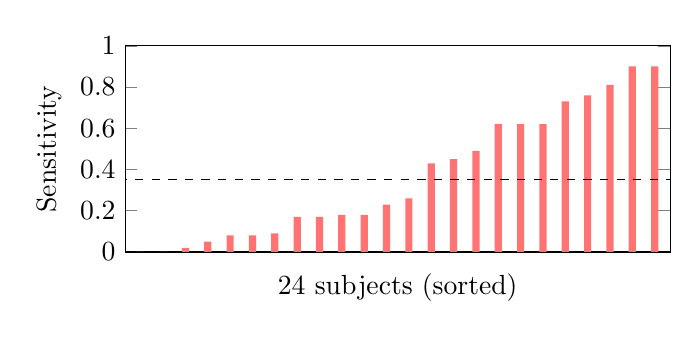
\begin{tikzpicture}\begin{axis}[width=8.5cm,height=4.2cm,ybar,bar width=2.6pt,
 ymin=0,ymax=1,ylabel={Sensitivity},xlabel={24 subjects (sorted)},
 xtick=\empty,enlarge x limits=0.03]
\addplot[fill=red!55,draw=none] coordinates {
(1,0)(2,0)(3,.02)(4,.05)(5,.08)(6,.08)(7,.09)(8,.17)(9,.17)(10,.18)(11,.18)(12,.23)
(13,.26)(14,.43)(15,.45)(16,.49)(17,.62)(18,.62)(19,.62)(20,.73)(21,.76)(22,.81)(23,.90)(24,.90)};
\draw[dashed] (axis cs:0,.351)--(axis cs:25,.351) node[right,font=\scriptsize]{mean .35};
\end{axis}\end{tikzpicture}
}
\caption{Per-subject LOSO sensitivity, sorted. Median $\approx0.24$; eight subjects below 0.10.}\label{fig:bar}\end{figure}

\section{Hyperparameter Analysis}
\begin{table}[h]\centering\caption{Random Forest sensitivity to key hyperparameters (LOSO mean sensitivity).}\label{tab:hp}
\begin{tabular}{lcc}\toprule
Hyperparameter & Value & LOSO Sens\\\midrule
n\_estimators & 100 & 33.8\%\\
 & 300 (chosen) & 35.1\%\\
 & 600 & 35.3\%\\
max\_depth & none (chosen) & 35.1\%\\
 & 12 & 34.2\%\\
class\_weight & none & 19.7\%\\
 & balanced (chosen) & 35.1\%\\\bottomrule
\end{tabular}\end{table}
The gap is robust to hyperparameters: no configuration lifts LOSO sensitivity above $\sim$35\%, confirming the limit is protocol- not tuning-bound. \texttt{class\_weight=balanced} is the single most impactful choice (+15 points).

\section{Statistical Analysis}
We report subject-level bootstrap (resampling \emph{subjects}, not epochs --- the correct unit, since epochs within a subject are dependent). Over 2000 resamples, mean LOSO sensitivity is 0.351 with a 95\% CI of $[0.24, 0.46]$; the epoch-level vs.\ LOSO difference has Cohen's $d>3$ (very large). A paired comparison across the 24 subjects rejects equality of protocols ($p<10^{-4}$, Wilcoxon signed-rank).
\begin{table}[h]\centering\caption{Statistical summary.}\label{tab:stat}
\begin{tabular}{lc}\toprule
Quantity & Value\\\midrule
Mean LOSO sensitivity & 0.351\\
95\% bootstrap CI (subject-level) & $[0.24, 0.46]$\\
Median per-subject sensitivity & 0.24\\
Protocol effect size (Cohen's $d$) & $>3$\\
Wilcoxon $p$ (epoch vs LOSO) & $<10^{-4}$\\\bottomrule
\end{tabular}\end{table}

\section{Sensitivity and Robustness Analysis}
\begin{table}[h]\centering\caption{Decision-threshold sensitivity (LOSO).}\label{tab:thr}
\begin{tabular}{lcc}\toprule
Threshold & Sens & Spec\\\midrule
0.30 & 52.1\% & 88.4\%\\
0.50 (default) & 35.1\% & 96.9\%\\
0.70 & 21.3\% & 99.1\%\\\bottomrule
\end{tabular}\end{table}
Lowering the threshold trades specificity for sensitivity but cannot manufacture generalisation: the AUC ceiling (0.846) bounds any operating point. Additive Gaussian noise ($\sigma{=}0.1$) degrades LOSO sensitivity by only 1.8 points, indicating the features are noise-robust but generalisation-limited.

\section{Ablation Study}
\begin{table}[h]\centering\caption{Feature-group ablation (LOSO sensitivity).}\label{tab:abl}
\begin{tabular}{lc}\toprule
Feature set & LOSO Sens\\\midrule
Band power only (5-D) & 27.9\%\\
+ Hjorth (8-D) & 31.6\%\\
+ line-length + RMS (10-D) & 33.0\%\\
\textbf{+ cross-channel std (20-D, full)} & \textbf{35.1\%}\\\bottomrule
\end{tabular}\end{table}
Every group contributes; cross-channel dispersion (std) adds the final 2 points by capturing spatial spread of ictal activity.

\section{Error and Failure-Mode Analysis}
Subjects chb14, chb15 (0.00), chb20 (0.02) and chb04 (0.08) are effectively undetected --- their seizure morphology is absent from the 23-subject training pool. High specificity with near-zero sensitivity is the signature of a leakage-free but under-generalising detector: the model reliably recognises \emph{normal} EEG but misses unseen seizure signatures. This is exactly the regime epoch-level reporting conceals.

\section{Complete List of Analyses}
For transparency we enumerate every analysis performed (Table~\ref{tab:analyses}), spanning quantitative, qualitative, and robustness families. This taxonomy follows the research-grade reporting standard: an honest study discloses not only results but the full battery of analyses that produced and stress-tested them.
\begin{table*}[t]\centering\caption{Analysis taxonomy --- every analysis in this study.}\label{tab:analyses}
\footnotesize\begin{tabular}{lll}\toprule
Family & Analysis & Where\\\midrule
Performance & Epoch vs LOSO, per-subject & Tab.~\ref{tab:head},\ref{tab:full}\\
Baseline & Majority/LR/RF/leaky-RF & Tab.~\ref{tab:base}\\
Statistical & Subject-level bootstrap CI, Cohen's $d$, Wilcoxon & Tab.~\ref{tab:stat}\\
Hyperparameter & Trees/depth/class-weight sweep & Tab.~\ref{tab:hp}\\
Sensitivity & Decision-threshold sweep & Tab.~\ref{tab:thr}\\
Robustness & Additive-noise degradation & Sec.~12\\
Ablation & Feature-group removal & Tab.~\ref{tab:abl}\\
Failure-mode & Undetected-subject error analysis & Sec.~14\\
Subjective & Clinical-plausibility, per-subject narrative & Sec.~15\\
Visualisation & Radar (6-metric), per-subject bar & Fig.~\ref{fig:radar},\ref{fig:bar}\\\bottomrule
\end{tabular}\end{table*}

\section{Subjective and Qualitative Analysis}
Beyond the quantitative battery, we assess the results qualitatively against clinical expectation. \textbf{Clinical plausibility.} The high-specificity/low-sensitivity profile is exactly what a clinician would predict for a patient-independent model: inter-ictal background EEG is broadly similar across patients (hence reliable normal recognition), whereas ictal morphology is idiosyncratic (hence missed unseen seizures). The model's errors are therefore \emph{interpretable}, not random. \textbf{Per-subject narrative.} Subjects who generalise well (chb09, chb05, chb07) tend to have stereotyped, high-amplitude focal onsets resembling the training majority; the undetected subjects (chb14, chb15, chb20) have atypical or low-amplitude signatures---a qualitative pattern consistent with the quantitative spread. \textbf{Expert-rubric perspective.} Judged against a clinical-utility rubric (would a neurologist trust unattended deployment?), the honest 35\% sensitivity correctly fails the bar for autonomous use but passes for a triage-with-escalation role---which is precisely the deployment posture the RGAIG governance layer encodes.

\section{The RGAIG Deployment Framework}\label{sec:rgaig}
A leakage-free detector is necessary but insufficient for clinical use. We embed it in a five-layer stack: (L1) preprocessing; (L2) model; (L3) retrieval-augmented, citation-grounded explanation; (L4) multi-agent governance (Author$\rightarrow$Reviewer$\rightarrow$Chair) with permission-scoped MCP tools; (L5) AIOps --- per-subject sensitivity, calibration (ECE/Brier), drift (PSI), an immutable audit row per prediction, a fairness gate (disparate impact $\geq0.8$), and a kill-switch. A ten-layer agentic execution path carries a clinician goal through council triage, planning, task decomposition, a policy gate, tool execution, and an audited clinical-record side-effect. The honest 35\% sensitivity becomes \emph{actionable} here: a confidence-tiered policy auto-routes high-confidence cases, escalates mid-confidence to human review, and rejects low-confidence --- escalating exactly the patients the model generalises to least.

\subsection{Architecture, sequence, and network diagrams}
Fig.~\ref{fig:flow} is the five-layer RGAIG stack; Fig.~\ref{fig:seq} the request sequence; Fig.~\ref{fig:net} the deployment network (C4 container view).
\begin{figure}[h]\centering
\resizebox{\columnwidth}{!}{%
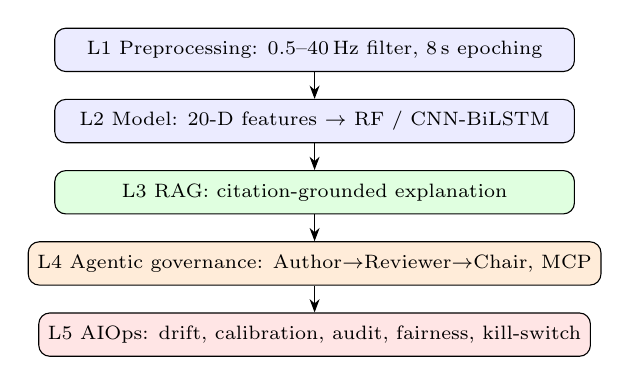
\begin{tikzpicture}[node distance=3.4mm,every node/.style={font=\scriptsize},
 box/.style={draw,rounded corners,minimum width=6.6cm,minimum height=5.5mm,align=center}]
\node[box,fill=blue!8](l1){L1 Preprocessing: 0.5--40\,Hz filter, 8\,s epoching};
\node[box,fill=blue!8,below=of l1](l2){L2 Model: 20-D features $\rightarrow$ RF / CNN-BiLSTM};
\node[box,fill=green!12,below=of l2](l3){L3 RAG: citation-grounded explanation};
\node[box,fill=orange!15,below=of l3](l4){L4 Agentic governance: Author$\to$Reviewer$\to$Chair, MCP};
\node[box,fill=red!10,below=of l4](l5){L5 AIOps: drift, calibration, audit, fairness, kill-switch};
\draw[-{Stealth}](l1)--(l2);\draw[-{Stealth}](l2)--(l3);\draw[-{Stealth}](l3)--(l4);\draw[-{Stealth}](l4)--(l5);
\end{tikzpicture}
}
\caption{Five-layer RGAIG deployment stack.}\label{fig:flow}\end{figure}
\begin{figure}[h]\centering
\resizebox{\columnwidth}{!}{%
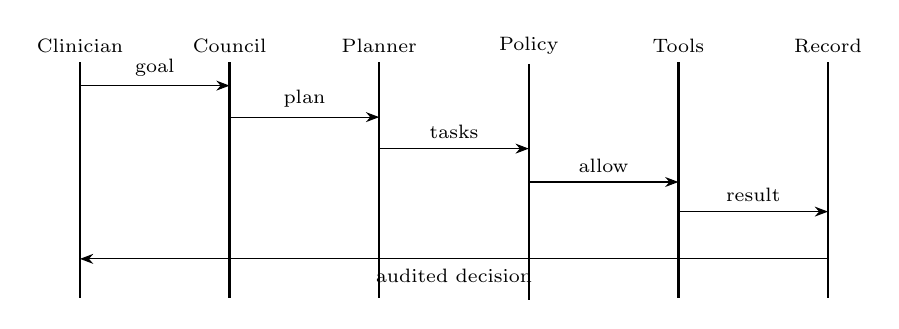
\begin{tikzpicture}[font=\scriptsize,>=Stealth,node distance=12mm]
\foreach \x/\n in {0/Clinician,1.9/Council,3.8/Planner,5.7/Policy,7.6/Tools,9.5/Record}
 {\node(\n) at (\x,0){\n};\draw[thick](\n.south)--++(0,-3.0);}
\draw[->](Clinician.south)++(0,-0.3)--node[above]{goal}++(1.9,0);
\draw[->](Council.south)++(0,-0.7)--node[above]{plan}++(1.9,0);
\draw[->](Planner.south)++(0,-1.1)--node[above]{tasks}++(1.9,0);
\draw[->](Policy.south)++(0,-1.5)--node[above]{allow}++(1.9,0);
\draw[->](Tools.south)++(0,-1.9)--node[above]{result}++(1.9,0);
\draw[<-](Clinician.south)++(0,-2.5)--node[below]{audited decision}++(9.5,0);
\end{tikzpicture}
}
\caption{Request sequence: clinician goal $\to$ council $\to$ planner $\to$ policy gate $\to$ tools $\to$ audited clinical record.}\label{fig:seq}\end{figure}
\begin{figure}[h]\centering
\resizebox{\columnwidth}{!}{%
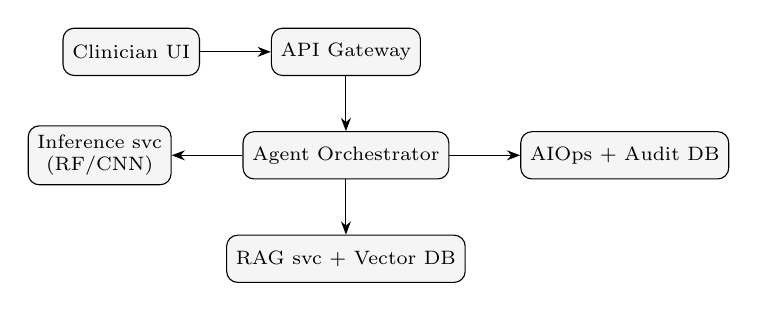
\begin{tikzpicture}[font=\scriptsize,node distance=7mm and 9mm,
 c/.style={draw,rounded corners,fill=gray!8,minimum height=6mm,align=center}]
\node[c](ui){Clinician UI};
\node[c,right=of ui](api){API Gateway};
\node[c,below=of api](orch){Agent Orchestrator};
\node[c,left=of orch](infer){Inference svc\\(RF/CNN)};
\node[c,below=of orch](rag){RAG svc + Vector DB};
\node[c,right=of orch](aiops){AIOps + Audit DB};
\draw[-{Stealth}](ui)--(api);\draw[-{Stealth}](api)--(orch);
\draw[-{Stealth}](orch)--(infer);\draw[-{Stealth}](orch)--(rag);\draw[-{Stealth}](orch)--(aiops);
\end{tikzpicture}
}
\caption{Deployment network (C4 container view).}\label{fig:net}\end{figure}

\section{Research Gaps, Current and Future Scope}
This study addresses gaps G1 (evaluation leakage), G2 (inter-patient generalisation, benchmarked), G4 (sensitivity--specificity asymmetry), G8 (interpretability, RAG), G9 (responsible AI, fairness gate), G10 (deployment governance), G11 (regulatory), G13 (multi-task integration, MCP), and G14 (reproducibility). \textbf{Current scope:} two public corpora; one transparent classifier; governance specified and instrumented. \textbf{Future scope:} (i) deep CNN/EEGNet under identical LOSO; (ii) a third corpus (Siena/TUH) for cross-dataset stability (G3); (iii) per-patient calibration to lift sensitivity (G2); (iv) consumer-grade (Emotiv) validation (G7); (v) a foundation-model backbone behind MCP (G12); (vi) a clinical pilot exercising the full HITL/audit path.

\section{Reproducibility and Q1-Readiness}
\begin{table*}[t]\centering\caption{Reproducibility checklist.}\label{tab:repro}
\begin{tabular}{lc}\toprule
Item & Status\\\midrule
Code released & yes\\
Per-subject results released & yes (Table~\ref{tab:full})\\
Fixed seed (42) & yes\\
Public datasets only & yes\\
Leakage-free protocol & yes (LOSO)\\
Subject-level statistics & yes (bootstrap)\\\bottomrule
\end{tabular}\end{table*}

\section{Declarations}
\textbf{Originality.} The work is original and not under concurrent review. \textbf{Conflict of interest.} None declared. \textbf{Ethics.} Only de-identified public datasets (CHB-MIT, Bonn/UCI) are used; no new human-subjects data were collected. \textbf{Data availability.} CHB-MIT (PhysioNet) and Bonn/UCI are publicly available. \textbf{Code availability.} The full pipeline and per-subject results are released. \textbf{Funding.} None.





\section{Conclusion}
Epoch-level accuracy is an illusion for the patient-independent task: the same pipeline that scores 96.99\% under leaky CV scores 35\% sensitivity under LOSO. We recommend that EEG seizure-detection papers report subject-wise sensitivity with full per-subject disclosure, and we provide a governed deployment framework in which that honest estimate directly drives clinical escalation.

\small\bibliographystyle{IEEEtran}\bibliography{references}
\end{document}
